\section{Inference}
\label{inf}

TRILL systems can answer many different queries. To do so, it exploits an algorithm called \emph{tableau} algorithm, which is able to collect explanations. In the following you can find an example that shows how the tableau works. In section~\ref{sec:trillq} we will see how queries can be asked with TRILL systems.

Consider a simple knowledge base inspired by the film ``The Godfather'' containing the following axioms:
\begin{align}
&tom : Cat\\
&(donVito, tom) : hasPet\\
&Cat \sqsubseteq Pet\\
&\exists hasAnimal.Pet \sqsubseteq NatureLover\\
&NatureLover \sqsubseteq GoodPerson\\
&hasPet \sqsubseteq hasAnimal
\end{align}

The axioms are telling what is known about the domain: (1) Tom is an individual of the domain, and he is a Cat; (2) donVito (Vito Corleone) has tom as his pet; (3) all cats are also pets; (4) everyone having at least one animal which is a pet is a nature lover; (5) nature lovers are good people; and (6) if one has a pet, she/he also has an animal.

This KB can be defined by the following TRILL syntax axioms:
\begin{verbatim}
classAssertion(cat, tom).
propertyAssertion(hasPet, donVito, tom).
subClassOf(cat, pet).
subClassOf(someValuesFrom(hasAnimal, pet), natureLover).
subClassOf(natureLover,goodPerson).
subPropertyOf(hasPet,hasAnimal).
\end{verbatim}
You can run this example \href{http://trill-sw.eu/example/trill/donVito.pl}{here}.

The first two axioms are assertional axioms (hence they constitute the ABox), the other four axioms define the TBox. Axiom 1 is called class assertion, 2 is called property assertion, 3,4,5 are called class subsumption axioms, and axiom 6 is called property subsumption axiom.

To check, for example, whether don Vito Corleone is a good person, the tableau algorithm builds a graph, called the \emph{tableau}. The initial tableau contains information from the ABox plus the negation of the query, as depicted in Figure\ref{fig:tab1}. This last axiom is added since the underlying proof mechanism uses refutation. In logic, working by refutation means assuming the opposite of the query one wants to prove. Then, if this assumption leads to a contradiction, this means that the axioms of the ontology allows to prove that the query is true, and thus that its opposite is false. In practice, working by refutation means that the graph must assume that the posed query be false, the tableau algorithm expands all the known axioms (including the negation of the query) and looks for contradictions present in the final graph. The presence of a contradiction in a node proves that the query is true because the graph depicts at least one way to contradict the negation of that query, and thus it depicts at least one way to prove that the opposite of the query contradicts what is defined by the ontology. 

\begin{figure}
	\centering
	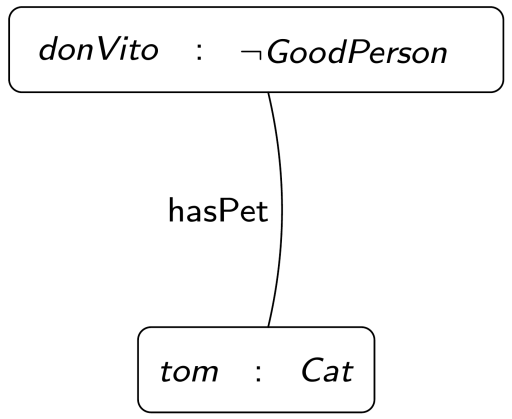
\includegraphics[width=0.5\linewidth]{img/tab1}
	\caption{Initial tableau}
	\label{fig:tab1}
\end{figure}

This means that if the opposite of the query is (artificially) added to the knowledge base as a new axiom, this ontology will contain at least two pieces of information one contradicting the other.

The tableau has one node for each individual: tom is labelled as cat, $donVito$ is labelled as not a good person (the negation of the query), and the edge between them is labelled as $hasPet$ because the individuals are connected by this property (Figure~\ref{fig:tab1}).

At this point, the graph of Figure~\ref{fig:tab1} is expanded using the axioms of the ontology to check the truth of the query and to build the justifications. Therefore, the tableau algorithm takes e.g. the axiom 3, ``cats are pets'', and adds to the node for tom also the label $pet$ since he is a cat. This new information is true and its justification is given directly by the set of axioms {1,3}: axiom 3 because since $tom$ is a $cat$ (axiom 1) he is also a $pet$. The same operation can be done for the edge (relationship) between tom and $donVito$, which can be labelled also as $hasAnimal$ because of axioms~2 and~6.

At this point, the calculus can deduce that $donVito$ belongs to the class \linebreak $\exists hasAnimal.Pet$ because $donVito$ is connected with $tom$, which is a $pet$ (axioms {1,3}), via property $hasAnimal$ (axioms {2,6}). Therefore, $donVito$’s node is labelled also as $\exists hasAnimal.Pet$ with a justification given by the union of the axioms associated with the used axioms, therefore its justification is given by the set of the involved axioms {1,2,3,6}. Then, the tableau graph is further expanded by adding the class $NatureLover$ to $donVito$’s node using axiom 4 and finally, by adding also the class $GoodPerson$ using label $NatureLover$ (axioms {1,2,3,4,6}) and axiom 5, creating as justification the set of axioms {1,2,3,4,5,6}.

The final graph is shown in Figure~\ref{fig:tab2}.
\begin{figure}
	\centering
	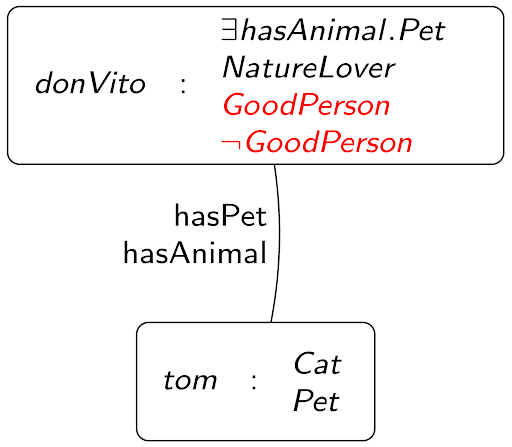
\includegraphics[width=0.5\linewidth]{img/tab2}
	\caption{Final tableau}
	\label{fig:tab2}
\end{figure}
The expanded graph contains now a contradiction, i.e., $donVito$ is labelled as $GoodPerson$ and as not a $GoodPerson$ (i.e., $\neg GoodPerson$), therefore, by refutation, the query ``Is don Vito Corleone a good person?'' is true, with justification given by the axioms {1,2,3,4,5,6}, that are the axioms of the KB necessary to deduce this information.

From this example, it would be clear why the use of probabilistic information is useful. Indeed, don Vito Corleone is hardly classifiable as a good person. This is because not all people who are nature lovers are also good, and therefore, one could say that axiom 5 is true with probability 0.4. It would also be arguable that everyone who has animals is also a nature lover, making probabilistic also this axiom. For a formal description of how the probability of the query is computed see the Appendix~\ref{app:inf}.